% !TEX TS-program = xelatex
% !TEX encoding = UTF-8 Unicode
% !Mode:: "TeX:UTF-8"

\documentclass{myresume}
\usepackage{zh_CN-Adobefonts_external} % Simplified Chinese Support using external fonts (./fonts/zh_CN-Adobe/)
%\usepackage{zh_CN-Adobefonts_internal} % Simplified Chinese Support using system fonts
\usepackage{linespacing_fix} % disable extra space before next section
\usepackage{cite}
\usepackage{graphicx}

\begin{document}
\pagenumbering{gobble} % suppress displaying page number

\begin{minipage}{0.65\textwidth}
\begingroup
\let\center\flushleft
\let\endcenter\endflushleft
\name{xxx}
\bigbreak
\phone{xxxxxxxxxxx}
\email{fengmengzhao@gmail.com}
\homepage{https://fmzhao.github.io}
\endgroup
\end{minipage}
\raggedleft{
\begin{minipage}{0.3\textwidth}
\flushright{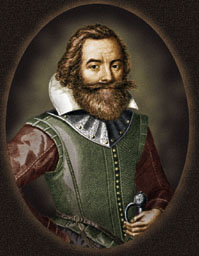
\includegraphics[width=58pt]{picture}}
\end{minipage}
}


% {E-mail}{mobilephone}{homepage}
% be careful of _ in emaill address
%\contactInfo{fengmengzhao@gmail.com}{(+86) 187-284-63725}{https://fmzhao.github.io}
% {E-mail}{mobilephone}
% keep the last empty braces!
%\contactInfo{xxx@yuanbin.me}{(+86) 131-221-87xxx}{}

\section{学历 \faGraduationCap}
\datedsubsection{\textbf{xxxx大学}\ 成都}{xxxx -- 至今}
\raggedleft{\fontsize{9pt}{11pt}{\textit{xxxx}\ xxxx \space xxxx}}
\datedsubsection{\textbf{xxxx大学}\ xxx}{xxxx -- xxxx}
\raggedleft{\fontsize{9pt}{11pt}{\textit{xx}\ xxxx}}

\bigbreak

\section{项目 \faGithub}

\datedsubsection{\textbf{DSA}}{2016年05月 -- 至今}
%\role{\LaTeX, Python}{个人项目}
\begin{onehalfspacing}
% 优雅的 \LaTeX\ 简历模板, https://github.com/billryan/resume
\raggedright{\fontsize{9pt}{11pt}{\textit{xxxxxxxxxxxxxxxxxxxxx}}}
\begin{itemize}
  \item xxxxxxxxxxxxxxxxxxxxx
  \item xxxxxxxxxxxxxxxxxxxxx
  \item xxxxxxxxxxxxxxxxxxxxx
  \item xxxxxxxxxxxxxxxxxxxxx
\end{itemize}
\end{onehalfspacing}

\datedsubsection{\textbf{机器学习}}{2016年03月 -- 2016月04月}
%\role{\LaTeX, Python}{个人项目}
\begin{onehalfspacing}
%优雅的 \LaTeX\ 简历模板, https://github.com/billryan/resume
\raggedright{\fontsize{9pt}{11pt}{\textit{xxxxxxxxxxxxxxxxxxxxx}}}
\begin{itemize}
  \item xxxxxxxxxxxxxxxxxxxxx
  \item xxxxxxxxxxxxxxxxxxxxx
  \item xxxxxxxxxxxxxxxxxxxxx
\end{itemize}
\end{onehalfspacing}

\datedsubsection{\textbf{Linux}}{2015年12月 -- 2016年02月}
%\role{\LaTeX, Python}{个人项目}
\begin{onehalfspacing}
%优雅的 \LaTeX\ 简历模板, https://github.com/billryan/resume
\raggedright{\fontsize{9pt}{11pt}{\textit{xxxxxxxxxxxxxxxxxxxxx}}}
\begin{itemize}
  \item xxxxxxxxxxxxxxxxxxxxx
  \item xxxxxxxxxxxxxxxxxxxxx
  \item xxxxxxxxxxxxxxxxxxxxx
  \item xxxxxxxxxxxxxxxxxxxxx
\end{itemize}
\end{onehalfspacing}

\datedsubsection{\textbf{Java EE}}{2015年08月 -- 2015年11月}
%\role{Golang, Linux}{个人项目,和富帅糕合作开发}
\begin{onehalfspacing}
\raggedright{\fontsize{9pt}{11pt}{\textit{xxxxxxxxxxxxxxxxxxxxx}}}
\begin{itemize}
  \item xxxxxxxxxxxxxxxxxxxxx
  \item xxxxxxxxxxxxxxxxxxxxx
  \item xxxxxxxxxxxxxxxxxxxxx
  \item xxxxxxxxxxxxxxxxxxxxx
\end{itemize}
\end{onehalfspacing}

\datedsubsection{\textbf{Jave SE}}{2015年04月 -- 2015年07月}
%\role{实习}{经理: 高富帅}
\raggedright{\fontsize{9pt}{11pt}{\textit{xxxxxxxxxxxxxxxxxxxxx}}}
\begin{itemize}
  \item xxxxxxxxxxxxxxxxxxxxx
  \item xxxxxxxxxxxxxxxxxxxxx
  \item xxxxxxxxxxxxxxxxxxxxx
  \item xxxxxxxxxxxxxxxxxxxxx
\end{itemize}

\section{IT 技能 \faCogs}
% increase linespacing [parsep=0.5ex]
\begin{itemize}[parsep=0.5ex]
  \item 编程语言:xxxx
  \item 优化:xxxx
  \item 平台:xxxx
  \item 版本控制:xxxx
  \item 建模语言:xxxx
  \item 数据库:xxxx
  \item 并发编程:xxxx
\end{itemize}

\bigbreak

\section{IT 兴趣 \faBug}
%\datedline{\textit{第一名}, xxx 比赛}{2013 年6 月}
%\datedline{其他奖项}{2015}
\begin{itemize}[parsep=0.5ex]
  \item xxxxxxxxxxxx
  \item xxxxxxxxxxxx
  \item xxxxxxxxxxxx
  \item xxxxxxxxxxxx
\end{itemize}

\bigbreak

\section{自我 \faAt}
% increase linespacing [parsep=0.5ex]
{\textbf{认知}}
\begin{onehalfspacing}
\begin{itemize}[parsep=0.5ex]
  \item xxxxxxxxxxxxxxxxxxxxxxxxxxxxxxxxxxxxxxxxxxxxxxxx
  \item xxxxxxxxxxxxxxxxxxxxxxxxxxxxxxxxxxxxxxxxxxxxxxxx
\end{itemize}
\end{onehalfspacing}

{\textbf{格言}}
\begin{onehalfspacing}
\begin{itemize}[parsep=0.5ex]
  \item xxxxxxxxxxxxxxxxxxxxxxxxxxxxxxxxxxxxxxxxxxxxxxxx
  \item xxxxxxxxxxxxxxxxxxxxxxxxxxxxxxxxxxxxxxxxxxxxxxxx
\end{itemize}
\end{onehalfspacing}

{\textbf{优点}
\begin{onehalfspacing}
\begin{itemize}[parsep=0.5ex]
  \item xxxx
  \item xxxx
  \item xxxx
\end{itemize}
\end{onehalfspacing}

{\textbf{缺点}
\begin{onehalfspacing}
\begin{itemize}[parsep=0.5ex]
  \item xxxxx
  \item xxxxx
\end{itemize}
\end{onehalfspacing}

{\textbf{爱好}
\begin{onehalfspacing}
\begin{itemize}[parsep=0.5ex]
  \item xx
  \item xx 
  \item xx
\end{itemize}
\end{onehalfspacing}

\end{document}
